%%%%%%%%%%%%%%%%%%%%%%%%%%%%%%%%%%%%%%%%%
% Masters/Doctoral Thesis 
% LaTeX Template
% Version 1.43 (17/5/14)
%
% This template has been downloaded from:
% http://www.LaTeXTemplates.com
%
% Original authors:
% Steven Gunn 
% http://users.ecs.soton.ac.uk/srg/softwaretools/document/templates/
% and
% Sunil Patel
% http://www.sunilpatel.co.uk/thesis-template/
%
% License:
% CC BY-NC-SA 3.0 (http://creativecommons.org/licenses/by-nc-sa/3.0/)
%
% Note:
% Make sure to edit document variables in the Thesis.cls file
%
%%%%%%%%%%%%%%%%%%%%%%%%%%%%%%%%%%%%%%%%% 

%----------------------------------------------------------------------------------------
%	PACKAGES AND OTHER DOCUMENT CONFIGURATIONS
%----------------------------------------------------------------------------------------

\documentclass[11pt, oneside]{Thesis} % The default font size and one-sided printing (no margin offsets)

\graphicspath{{Pictures/}} % Specifies the directory where pictures are stored

\usepackage[comma, sort&compress]{natbib} % Use the natbib reference package - read up on this to edit the reference style; if you want text (e.g. Smith et al., 2012) for the in-text references (instead of numbers), remove 'numbers' 

%\usepackage{booktabs}
\usepackage{array}
%\usepackage{apacite}

\newcolumntype{x}[1]
            {>{\raggedright}p{#1}}
\newcommand{\tn}{\tabularnewline}

\hypersetup{urlcolor=blue, colorlinks=true} % Colors hyperlinks in blue - change to black if annoying
\title{\ttitle} % Defines the thesis title - don't touch this

\begin{document}

\frontmatter % Use roman page numbering style (i, ii, iii, iv...) for the pre-content pages

\setstretch{1.3} % Line spacing of 1.3

% Define the page headers using the FancyHdr package and set up for one-sided printing
\fancyhead{} % Clears all page headers and footers
\rhead{\thepage} % Sets the right side header to show the page number
\lhead{} % Clears the left side page header

\pagestyle{fancy} % Finally, use the "fancy" page style to implement the FancyHdr headers

\newcommand{\HRule}{\rule{\linewidth}{0.5mm}} % New command to make the lines in the title page

% PDF meta-data
\hypersetup{pdftitle={\ttitle}}
\hypersetup{pdfsubject=\subjectname}
\hypersetup{pdfauthor=\authornames}
\hypersetup{pdfkeywords=\keywordnames}

%----------------------------------------------------------------------------------------
%	TITLE PAGE
%----------------------------------------------------------------------------------------

\begin{titlepage}
\begin{center}

\textsc{\LARGE \univname}\\[1.5cm] % University name
\textsc{\Large Doctoral Thesis}\\[0.5cm] % Thesis type

\HRule \\[0.5cm] % Horizontal line
{\huge \bfseries \ttitle}\\[0.4cm] % Thesis title
\HRule \\[1.5cm] % Horizontal line

\begin{minipage}{0.4\textwidth}
\begin{flushleft} \large
\emph{Author:}\\
\href{http://www.johnsmith.com}{\authornames} % Author name - remove the \href bracket to remove the link
\end{flushleft}
\end{minipage}
\begin{minipage}{0.4\textwidth}
\begin{flushright} \large
\emph{Supervisor:} \\
\href{http://www.jamessmith.com}{\supname} % Supervisor name - remove the \href bracket to remove the link  
\end{flushright}
\end{minipage}\\[3cm]
 
\large \textit{A thesis submitted in fulfilment of the requirements\\ for the degree of \degreename}\\[0.3cm] % University requirement text
\textit{in the}\\[0.4cm]
\groupname\\\deptname\\[2cm] % Research group name and department name
 
{\large \today}\\[4cm] % Date
%\includegraphics{Logo} % University/department logo - uncomment to place it
 
\vfill
\end{center}

\end{titlepage}

%----------------------------------------------------------------------------------------
%	DECLARATION PAGE
%	Your institution may give you a different text to place here
%----------------------------------------------------------------------------------------

\Declaration{

\addtocontents{toc}{\vspace{1em}} % Add a gap in the Contents, for aesthetics

I, \authornames, declare that this thesis titled, '\ttitle' and the work presented in it are my own. I confirm that:

\begin{itemize} 
\item[\tiny{$\blacksquare$}] This work was done wholly or mainly while in candidature for a research degree at this University.
\item[\tiny{$\blacksquare$}] Where any part of this thesis has previously been submitted for a degree or any other qualification at this University or any other institution, this has been clearly stated.
\item[\tiny{$\blacksquare$}] Where I have consulted the published work of others, this is always clearly attributed.
\item[\tiny{$\blacksquare$}] Where I have quoted from the work of others, the source is always given. With the exception of such quotations, this thesis is entirely my own work.
\item[\tiny{$\blacksquare$}] I have acknowledged all main sources of help.
\item[\tiny{$\blacksquare$}] Where the thesis is based on work done by myself jointly with others, I have made clear exactly what was done by others and what I have contributed myself.\\
\end{itemize}
 
Signed:\\
\rule[1em]{25em}{0.5pt} % This prints a line for the signature
 
Date:\\
\rule[1em]{25em}{0.5pt} % This prints a line to write the date
}

\clearpage % Start a new page

%----------------------------------------------------------------------------------------
%	QUOTATION PAGE
%----------------------------------------------------------------------------------------

\pagestyle{empty} % No headers or footers for the following pages

\null\vfill % Add some space to move the quote down the page a bit

\textit{``Thanks to my solid academic training, today I can write hundreds of words on virtually any topic without possessing a shred of information, which is how I got a good job in journalism."}

\begin{flushright}
Dave Barry
\end{flushright}

\vfill\vfill\vfill\vfill\vfill\vfill\null % Add some space at the bottom to position the quote just right

\clearpage % Start a new page

%----------------------------------------------------------------------------------------
%	ABSTRACT PAGE
%----------------------------------------------------------------------------------------

\addtotoc{Abstract} % Add the "Abstract" page entry to the Contents

\abstract{\addtocontents{toc}{\vspace{1em}} % Add a gap in the Contents, for aesthetics

The Thesis Abstract is written here (and usually kept to just this page). The page is kept centered vertically so can expand into the blank space above the title too\ldots
}

\clearpage % Start a new page

%----------------------------------------------------------------------------------------
%	ACKNOWLEDGEMENTS
%----------------------------------------------------------------------------------------

\setstretch{1.3} % Reset the line-spacing to 1.3 for body text (if it has changed)

\acknowledgements{\addtocontents{toc}{\vspace{1em}} % Add a gap in the Contents, for aesthetics

The acknowledgements and the people to thank go here, don't forget to include your project advisor\ldots
}
\clearpage % Start a new page

%----------------------------------------------------------------------------------------
%	LIST OF CONTENTS/FIGURES/TABLES PAGES
%----------------------------------------------------------------------------------------

\pagestyle{fancy} % The page style headers have been "empty" all this time, now use the "fancy" headers as defined before to bring them back

\lhead{\emph{Contents}} % Set the left side page header to "Contents"
\tableofcontents % Write out the Table of Contents

\lhead{\emph{List of Figures}} % Set the left side page header to "List of Figures"
\listoffigures % Write out the List of Figures

\lhead{\emph{List of Tables}} % Set the left side page header to "List of Tables"
\listoftables % Write out the List of Tables

%----------------------------------------------------------------------------------------
%	ABBREVIATIONS
%----------------------------------------------------------------------------------------

\clearpage % Start a new page

\setstretch{1.5} % Set the line spacing to 1.5, this makes the following tables easier to read

\lhead{\emph{Abbreviations}} % Set the left side page header to "Abbreviations"
\listofsymbols{ll} % Include a list of Abbreviations (a table of two columns)
{
\textbf{LAH} & \textbf{L}ist \textbf{A}bbreviations \textbf{H}ere \\
%\textbf{Acronym} & \textbf{W}hat (it) \textbf{S}tands \textbf{F}or \\
}

%----------------------------------------------------------------------------------------
%	PHYSICAL CONSTANTS/OTHER DEFINITIONS
%----------------------------------------------------------------------------------------

\clearpage % Start a new page

\lhead{\emph{Physical Constants}} % Set the left side page header to "Physical Constants"

\listofconstants{lrcl} % Include a list of Physical Constants (a four column table)
{
Speed of Light & $c$ & $=$ & $2.997\ 924\ 58\times10^{8}\ \mbox{ms}^{-\mbox{s}}$ (exact)\\
% Constant Name & Symbol & = & Constant Value (with units) \\
}

%----------------------------------------------------------------------------------------
%	SYMBOLS
%----------------------------------------------------------------------------------------

\clearpage % Start a new page

\lhead{\emph{Symbols}} % Set the left side page header to "Symbols"

\listofnomenclature{lll} % Include a list of Symbols (a three column table)
{
$a$ & distance & m \\
$P$ & power & W (Js$^{-1}$) \\
% Symbol & Name & Unit \\

& & \\ % Gap to separate the Roman symbols from the Greek

$\omega$ & angular frequency & rads$^{-1}$ \\
% Symbol & Name & Unit \\
}

%----------------------------------------------------------------------------------------
%	DEDICATION
%----------------------------------------------------------------------------------------

\setstretch{1.3} % Return the line spacing back to 1.3

\pagestyle{empty} % Page style needs to be empty for this page

\dedicatory{For/Dedicated to/To my\ldots} % Dedication text

\addtocontents{toc}{\vspace{2em}} % Add a gap in the Contents, for aesthetics

%----------------------------------------------------------------------------------------
%	THESIS CONTENT - CHAPTERS
%----------------------------------------------------------------------------------------

\mainmatter % Begin numeric (1,2,3...) page numbering

\pagestyle{fancy} % Return the page headers back to the "fancy" style

% Include the chapters of the thesis as separate files from the Chapters folder
% Uncomment the lines as you write the chapters

% Chapter 1

\chapter{Methodology} % Main chapter title

\label{methodologychapter} % For referencing the chapter elsewhere, use \ref{Chapter1} 

\lhead{Chapter 1. \emph{Research Findings}} % This is for the header on each page - perhaps a shortened title

%----------------------------------------------------------------------------------------
\section{Preliminary Contextual Inquiry}
\subsection{Description of the Study}
The main objective of collecting preliminary contextual information was to elicit requirements to inform the design of a health self-monitoring application operated through intermediaries.  I had obtained ethics approval from Human Research Ethics Committee of Faculty of Health Sciences at University of Cape Town. I and one research assistant recruited participants at the diabetic and endocrine clinic located at Groote Schuur hospital in Cape Town. This is an outpatient clinic which runs on Thursdays and Fridays.\newline
Majority of the participants we recruited were above mid-aged. The rationale for choosing this group of participants was based on the fact that the technology I had envisaged to develop was targeting users who are less knowledgeable in cellphones and technology in general, therefore this group of participants was a representative of prospective beneficiary users of such a technology. My objective was to interview only overweight and obese patients but we also included few participants who appeared to be thin but were diabetic. Since diabetes is a lifestyle related disease, I found that it would be interesting to also understand utilization of cellphones, and access to information even to individuals who appear not to be overweight but these individuals may give out insights on various issues related technology utilization, and barriers to adoption of behaviors that are considered to be healthy.\newline
\subsection{Methods}
I together with my research assistant approached individual participants and explained the purpose of the study. People who agreed to participate were given consent forms to sign. We used a semi structured questionnaire attached at Appendix A to interview participants. Each participant was interviewed for a period of 20 to 30 minutes. The questionnaire had four groups of questions and these included demographics; cellphone ownership and utilization; access to health information and pedometers; and barriers to diet and physical activity.We interviewed a total of thirty participants.We started interviews in March 2013 and concluded at the beginning of May 2013. I analyzed quantitative data using descriptive statistics. I also examined qualitative data by extracting thematic areas which were key to informing the design of the prototype I had envisaged.\newline
\section{Implementation of the First Prototype of a Health Self-Monitoring Application}
\subsection{Implementation Platform}
I spent time developing an application based on findings from the aforementioned contextual inquiry. I was faced with a decision of whether to develop a native mobile application or web application. I decided to choose a web application. The rationale for choosing a web application was based on the following factor, I anticipated that users at evaluation stage were going to use their own mobile devices.\newline
I started developing the prototype using Django Python, Mobile Jquery, HTML 5.0, and MySQL. On the server side everything was implemented using Django Python and MySQL as the database. There were some limitations with this approach as not everything could be done on a web application. One draw back was a pedometer which required a native implementation because one has to implement code to interact with an accelerometer sensor which is platform dependent. Initially the plan was to find an off the shelf pedometer with an open API (Application Programming Interface). I came across a device called Fitbit\footnote{ https://www.fitbit.com/}. It has a RESTful\footnote{http://www.w3.org/TR/ws-arch/} web API that one could use to transfer steps' data to the Internet. I was unable to adopt Fitbit because it was not going to work in the context of participants I planned to recruit. Fitbit device required one to have a personal computer and a high end smart phone such as Samsung Galaxy III.\newline
I made a decision to implement a pedometer application that runs on android phones. I used open source code found on the Internet. This pedometer was capable of capturing steps walked by an individual and transfer them to the web application.\newline
\subsection{Implemented Features}
I developed a prototype that had the following features (screenshots are attached at appendix B):
\begin{itemize}
\item{Steps walked display at intervals of days, weeks, or months.}
\item{Recording of meals eaten specified by portions of food groups i.e. Lunch(fruits and vegetables,starch,dairy,fat,and high sugar food).}
\item{Meals charts showing the overall summary of each food consumed in intervals of days, weeks, or months.}
\item{Goal Setting that enables users to specify their desired targets in meals and steps walked.}
\item{A Reward sub-component(system) implemented using aquariums, botanical garden, leader boards integrated points and badges }
\end{itemize}
The premise of the aforementioned reward system was to engage users by supporting their motivation affordances\citep{zhang2008motivational} to engage with the prototype. I drew the design inspiration from a Self-Determination Theory (SDT)\citep{deci1985intrinsic}. SDT postulates that in order to support individuals intrinsic motivation needs you have to support three basic psychological needs which are perceived autonomy, perceived competence, and perceived relatedness. 

The prototype linked the reward system with Facebook social plugins that allow users to comment on or like each other. The idea was to allow each pair of users (an intermediary and beneficiary) to improve their relatedness with respect to other pairs of users. I also integrated a feedback mechanism that would appear on a Facebook group that comprises of all intermediary users as members. 


\section{Pilot Evaluation I}
\subsection{Description of the Study}
The plan was to evaluate the first version of the prototype with patients in  hospital settings. This plan didn't materialize since it was going to be arduous to negotiate ethics as far as the scientific contribution is concerned. One of the conditions for the study to go forward was to ensure that I carry it out as an RCT(Randomized Control Trial) with clinical or health outcomes afterwards. I had to redesign the study so that I work with participants outside of the hospital settings. I obtained a different ethics approval from FSREC(Faculty of Science Research Ethics Committee) of University of Cape Town.\newline
I recruited participants to help in evaluating an application through an NGO called Mamelani Projects\footnote{http://www.mamelani.org.za/} in Cape Town. This NGO works on  community health programs that target youth and women inhabiting in marginalized areas in the outskirts of Cape Town. Recruitment took place in September 2014. The NGO linked me with participants from a Township called Phillipi in Cape Town. A township in South African context is a suburb which is mostly inhabited by previously disadvantaged populations from an apartheid government. Phillipi township has both formal and informal settlements.  
\subsection{Methods}
 I recruited a total of six mid-aged women (35-45 years of age) to be beneficiary users of the prototype. These beneficiary participants came together with their family members to act as their intermediaries. The oldest intermediary was 23 years of age. Each beneficiary participant formed of a pair with their respective intermediary participant. I explained to participants of what they are expected to do. All twelve participants(6 intermediaries and six beneficiaries) signed informed consent and assent forms. After the signing of forms, I spent time teaching intermediaries on how to use the application. After the training intermediary participants I left participants with the application to use from the beginning of October 2014 to the end of November 2014  
\section{Second Iteration of Prototype Development}
After evaluation of the aforementioned first prototype, I did the second iteration of prototype development. This entailed fixing of bugs discovered during testing of the first prototype, and improvement of software functionality to closely emulate support for competition, autonomy, and relatedness. I revamped the prototype not to rely too much on Facebook as they were challenges in utilization of Facebook by participants. Some intermediaries had never used Facebook before, and the rest who were using Facebook, didn't utilize it so frequent hence reminders and other forms of feedback were not timely received by both intermediaries and beneficiaries. I opted to utilize SMS reminders in the second prototype. In addition, the township where I carried the first pilot evaluation had poor Internet signal and this affected accessibility of Facebook social features that were embedded in the app. Therefore, I designed my own social features to allow users to comment on or send messages to each other. This improved the ability of the app to load much faster as it didn't require any third party's plugins to load.
\section{Pilot Evaluation II} 
\subsection{Description of the Study}
Endeavours to continue working with participants from Phillipi were futile as I was advised to stop the recruitment process by the NGO I was working with. This was due to concerns that experimental phones were going to pose risk to both participants and the researcher. Therefore, in the second pilot evaluation, I had to find participants from Langa township which was more safer compared to Phillipi. I worked with a research assistant who was a resident of Langa. The research assistant helped with recruitment and screening of participants to identify the ones that met inclusion criteria to be recruited as participants. This time I had adjusted recruitment criteria after reflecting on the success and failure of the application deployed during the aforementioned first pilot evaluation. In the the evaluation of prototype I observed that it was nearly impossible for the intervention to have an impact if members of a pair don't cohabit or live within a proximity from each other. Therefore, this time I made a decision to only recruit beneficiary users who would elect intermediaries that are related to them and live nearby or in the same house with them. 
\subsection{Data Collection Methods}
\subsubsection{Interviews}

\begin{flushright}
\end{flushright}

% Chapter 1

\chapter{Findings} % Main chapter title

\label{findingschapter} % For referencing the chapter elsewhere, use \ref{Chapter1} 

\lhead{Chapter 1. \emph{Research Findings}} % This is for the header on each page - perhaps a shortened title

%----------------------------------------------------------------------------------------

\section{Pilot Evaluation II Findings}
\subsection{Baseline}
We had a total of sixteen participants who completed the baseline questionnaire. There were two sets of participants. The first set consisted of seven beneficiaries while the second set consisted of nine intermediaries. At baseline level, findings are both in form of descriptive and inferential statistics. These findings focus on comparison between participants' characteristics from the two aforementioned sets.  \newline
At baseline, I examined three out of five variables, and these were age of participants, number of services/applications utilized by each participant, and intrinsic motivation to use cellphone. Other variables only existed in one group, therefore lacked comparative basis. The findings based on these variables is reported at mid-line and end-line points sections. \newline
Table \ref{table:ageDist} shows the mean age with its respective standard deviation for each set of participants. Beneficiaries had a mean age of 48 years old (SD: 7.9 years) while intermediaries had a mean age of 14 years (SD: 4.3 years).
\newline
\begin{table}[h!]
  \begin{center}
    \caption{Age distribution of two sets of participants at baseline.}
    \label{table:ageDist}
	\begin{tabular}{|r|r|r|r|}
		\hline
		Types of Users& Sample Size (n)& Mean age& Standard Deviation\\
		\hline
		Beneficiary Users& 7& 48.29& 7.910\\
		\hline
		Intermediary Users& 9& 14.00& 4.272\\
		\hline
	\end{tabular}
  \end{center}
\end{table}
\newline
The distribution of age in both sets was normal. I conducted a student t test to compare means of age from the two sets(groups). The mean age of intermediaries' set was significantly lower (M=14 ; SD=4.27) years compared to beneficiaries' set(M= 48.29; SD=7.910) years with (t(14)=11.148; p$<$0.01; 95\% CI= -40.88 to -27.69 years ). The mean difference in age was 34.28 years with a standard error of 3.08 years.
\newline
As part of the baseline questionnaire, I provided a list of names of cellphone based services/applications(apps) for participants to choose from. The words applications and services are used interchangeably throughout this chapter. The list contained ten services as demonstrated on Table \ref{table:servTab}. This list is not exhaustive but it attempted to capture most services that are considered to be prevalent.  
\begin{table}[h!]
  \begin{center}
    \caption{List of services/apps in the baseline questionnaire.}
    \label{table:servTab}
{ \renewcommand{\arraystretch}{1.2}
\begin{tabular}{|l|x{2cm}|x{10cm}|}
\hline
{}& \textbf{Service name}& \textbf{Description and purpose}\tn \hline
         1& SMS& SMS stands for short messaging service. It is one of the basic feature in every phone It is used for communication purposes \tn \hline
         2& Downloading& It is an Internet based service of where people download files such as music and video.\tn \hline
         3& WhatsAPP& Internet based messaging application.It is used for communication purposes \tn \hline
		 4& BBM& Internet based messaging application typically found in blackberry phones. It is used for communication purposes \tn \hline
		 5& WhatsAPP& Internet based messaging application. It is used for communication purposes \tn \hline
		 6& Facebook& Internet based social network platform which enables individuals to have social interactions \tn \hline
		 7& Twitter& Internet based social network platform which enables individuals to have social interactions \tn \hline
		 8& Email& It is an Internet based platform that allows individuals to have formal or informal communication. \tn \hline
		9& Pedometer& It refers to a specialized device or an application installed on mobile devices such as
		cellphones. Its purpose is to sense bodily movements. It is has to be attached to a person's body typically on the waist or at the front pocket of a trouser. An advanced pedometer can transfer detected movements via Internet or Bluetooth. It is recommended for tracking exercise or activity routines. \tn \hline
		10& Diary for Diet& It refers to an electronic journal that can be used to track meals eaten and probably provide summaries on which users can reflect on. It can installed either on stationary medium such as a personal computer or mobile devices such as cellphones, tablets, PDAs etc. \tn \hline
\end{tabular} }
 \end{center}
\end{table}
\newline Each participant selected services/app they have either interacted with before or they are knowledgeable with. Figure \ref{figure:OverallSerBase} indicates that SMS and Camera were the most prevalent with comparison to the remaining applications or services considering the number of participants that were using them. All sixteen participants indicated that they had interacted with both SMS and Camera before
\begin{figure}[htbp]
  \centering
    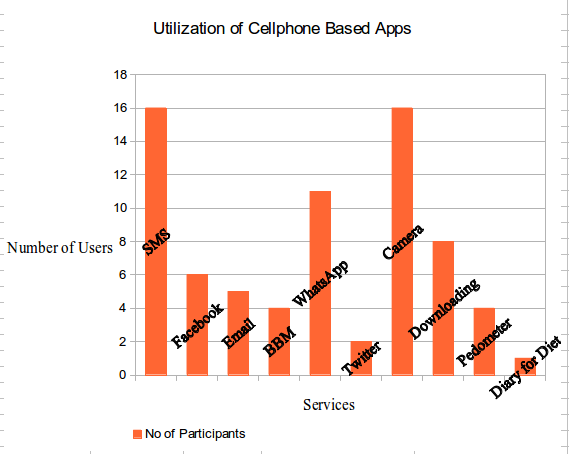
\includegraphics[width=0.8\textwidth]{Figures/overallcellphoneusebaseline.png}
    \rule{35em}{0.5pt}
  \caption{Average utilization of services and apps by the two groups of participants.}
  \label{figure:OverallServBase}
\end{figure}
\begin{figure}[htbp]
  \centering
    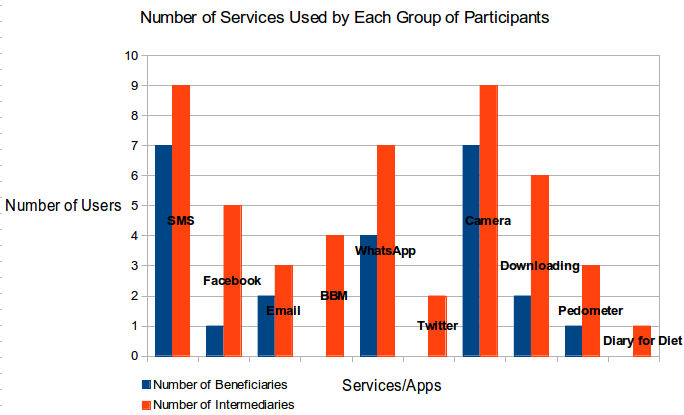
\includegraphics[width=0.8\textwidth]{Figures/baselinepilotallservices.png}
    \rule{35em}{0.5pt}
  \caption{Average utilization of services and apps by the two groups of participants.}
  \label{figure:AllServBase}
\end{figure}
I conducted a further analysis that compares the number of services the two groups of participants have interacted with before. Figure \ref{figure:AllServBase} shows the number of participants from each set that have interacted with each of the aforementioned services on Table \ref{table:servTab} above.
Figure \ref{figure:AllServBase} was not a good indicator of any differences between the two sets because the two samples differed in their sizes. I made a decision to only compare the averages of number of services used by each group of participants. Figure \ref{figure:AvgServBase}  shows that there is a difference on the averages of number of services that intermediaries have interacted with compared to the number of services beneficiaries have interacted with.
\begin{figure}[htbp]
  \centering
    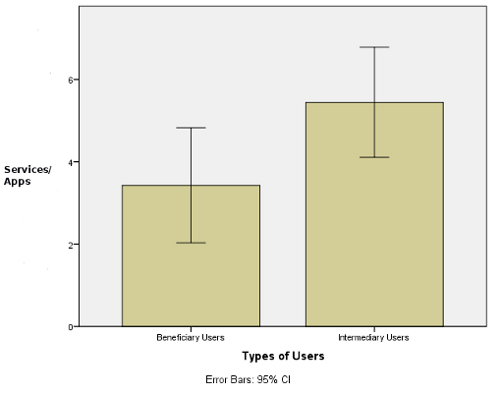
\includegraphics[width=0.8\textwidth]{Figures/ServicesBaseline.png}
    \rule{35em}{0.5pt}
  \caption{Average utilization of services and apps by the two groups of participants.}
  \label{figure:AvgServBase}
\end{figure}
A further inferential analysis by using a student t test indicated that intermediary participants had significantly interacted with more applications (M=5.44; SD=1.74) applications more of the aforementioned services compared to beneficiary users (M=3.43; SD=1.51) applications (t(14)=2.430; p=0.029; 95\% CI=3.765 to 3.795 applications). Due to a small sample size, I was unable to conduct a statistical test to compare the average usage of each service/application between intermediary and beneficiary participants.\newline
The above findings on average number of apps used by each group of participants suggest that our intermediary participants are more likely to interact with more services or applications compared to our beneficiary participants. These findings were in consensus with the observed difference in intrinsic motivation to use cellphone between the two groups. Figure 2 below shows a cluster bar chart for each scale I used for calculating the overall "{\textbf{\emph{intrinsic motivation to use cellphone}}". Figure \ref {figure:IMIScales} presents a descriptive visualization of differences in individual scales of intrinsic motivation to use cellphone in between intermediaries and beneficiaries.    
\begin{figure}[htbp]
  \centering
    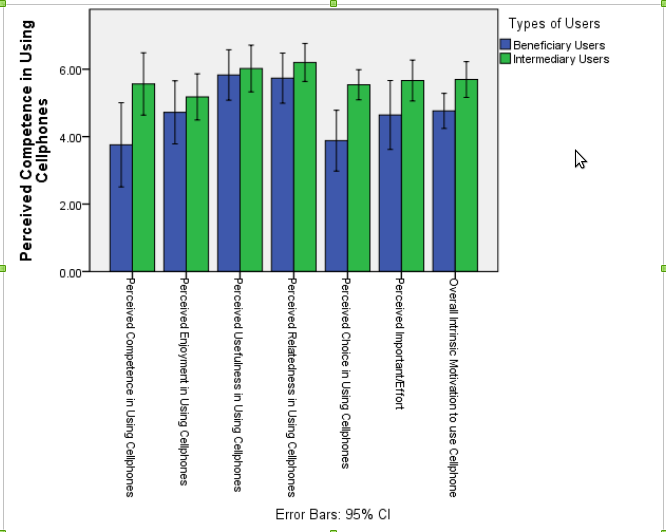
\includegraphics[width=0.8\textwidth]{Figures/IMIScales.png}
    \rule{35em}{0.5pt}
  \caption{Average utilization of services and apps by the two groups of participants.}
  \label{figure:IMIScales}
\end{figure}  
I conducted a student t-test to examine whether intermediaries and beneficiaries had significant differences on both scores from individual scales and overall intrinsic motivation. On scores of individual scales,  the differences were not significant in perceived enjoyment; perceived usefulness; and perceived relatedness. There were significant differences on the following scales; perceived competence; perceived choice; and perceived effort. Intermediaries scored significantly higher on perceived competence to use cellphones (M=5.5611 ;SD=1.20254) compared to beneficiaries (M=3.7571 ;SD=1.35106) with conditions;(t(14)=2.822 ; p=0.014 ; 95\% CI=0.43307 to 3.17486). Intermediaries' perception on self autonomy(perceived choice) to use cellphone (M=5.5378 ;SD=0.57933 ) was significantly higher compared to beneficiaries' perceived choice to use cellphone (M=3.8814;SD=0.97472) with conditions (t(14)=4.247; p=0.001; 95\% CI=0.81984  to 2.49286 ). Also intermediaries (M=5.6633; SD=0.78889) scored significantly higher on perceived effort/important compared to beneficiaries (M=4.6429 ;SD=1.10583) with conditions (t(14)=2.159; p=0.049; 95\% CI=0.00670 to 2.03426).\newline
On comparison between an overall intrinsic motivation scores to use cellphone between the two groups, intermediaries(M=5.6944 ;SD=0.69013 ) scored significantly higher than beneficiaries(M=4.7629 ;SD=0.56287) with conditions (t(14)=2.894; p=0.012; 95\% CI=0.24123 to 1.62194).These findings indicate that intermediary participants were more intrinsically motivated to engage with cellphones compared to beneficiary participants.
\begin{flushright}
\end{flushright}

%\input{Chapters/Chapter3}
%\input{Chapters/Chapter4} 
%\input{Chapters/Chapter5} 
%\input{Chapters/Chapter6} 
%\input{Chapters/Chapter7} 

%----------------------------------------------------------------------------------------
%	THESIS CONTENT - APPENDICES
%----------------------------------------------------------------------------------------

\addtocontents{toc}{\vspace{2em}} % Add a gap in the Contents, for aesthetics

\appendix % Cue to tell LaTeX that the following 'chapters' are Appendices

% Include the appendices of the thesis as separate files from the Appendices folder
% Uncomment the lines as you write the Appendices

%% Appendix A

\chapter{Appendix A. Ethics Approval -- Faculty of Health Sciences} % Main appendix title
\clearpage
\label{AppendixA} % For referencing this appendix elsewhere, use \ref{AppendixA}

\lhead{Appendix A. \emph{Ethics Approval -- Faculty of Health Sciences}} % This is for the header on each page - perhaps a shortened title
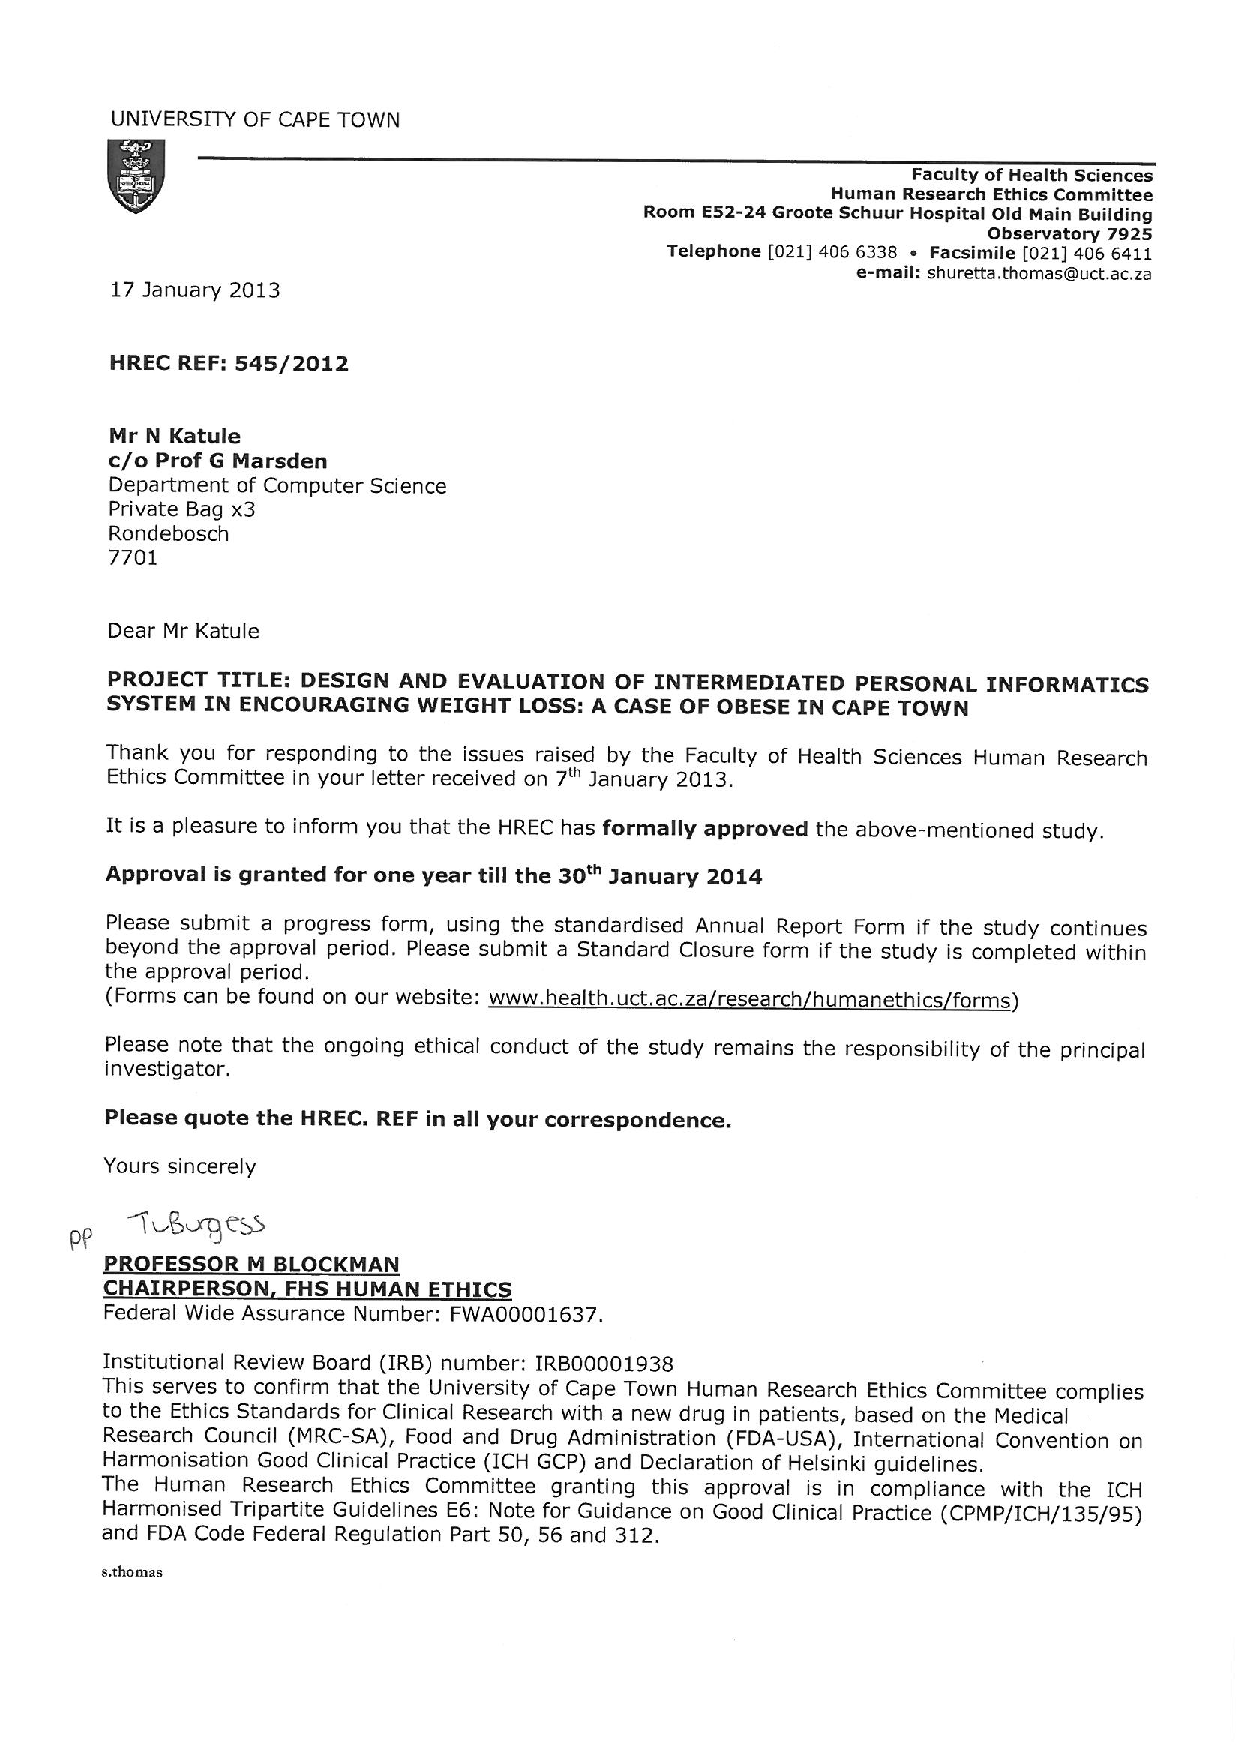
\includepdf[pages=-,pagecommand={},width=\textwidth,offset=90 -20]{Pdfs/fhsrec.pdf}

%\newcommand{\insertrep}[1]{%
%\hspace{-2.4cm}
%\fbox{\includegraphics[page=1,scale=0.8]{#1}}
%\includegraphics[page=1,scale=0.8]{#1}
%\includepdf[scale=0.75,pages=1,frame]{#1}
%}

%\subsection{Interesting Letter}
%\insertrep{Pdfs/baseline_ben.pdf}
%\begin{center}
%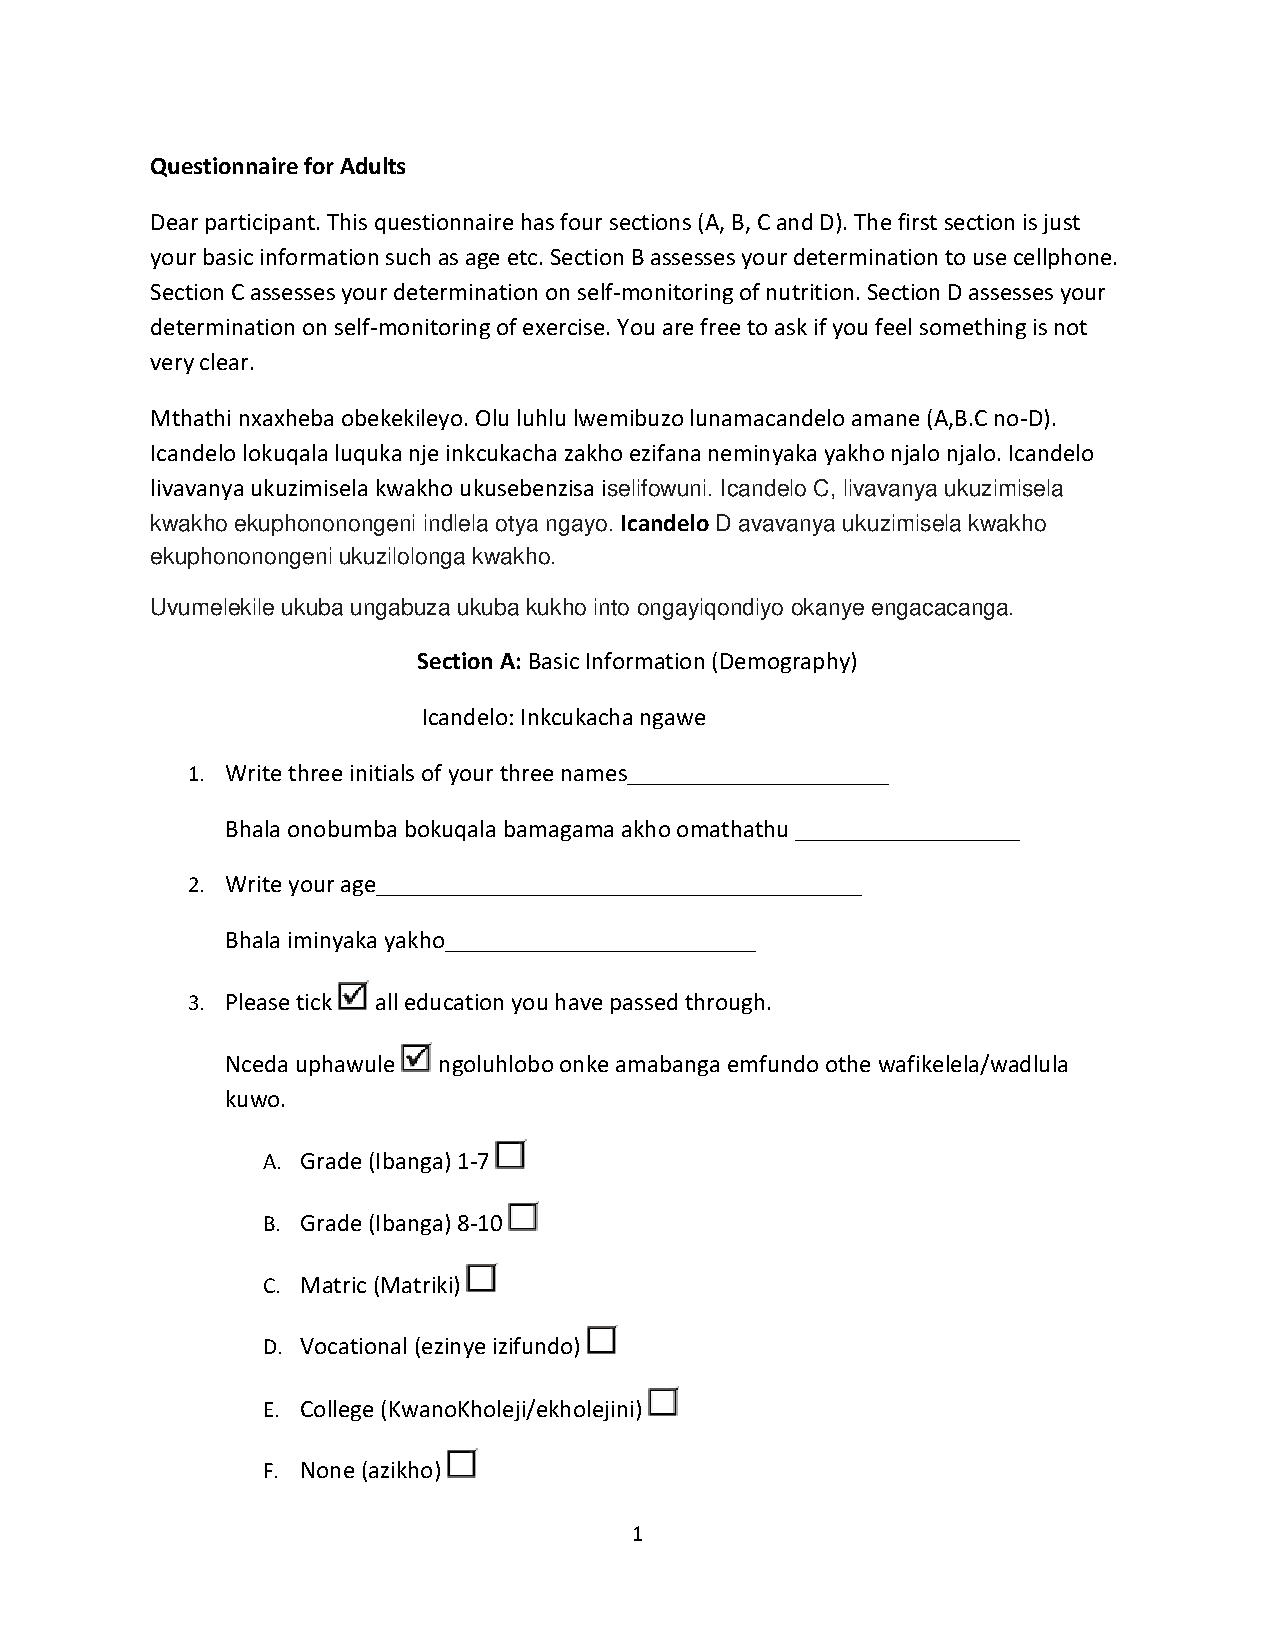
\includepdf[pagecommand={},scale=0.9]{Pdfs/baseline_ben.pdf} 
%\end{center}

%% Appendix A

\chapter{Appendix B. Ethics Approval -- Faculty of Science} % Main appendix title
\clearpage
\label{AppendixB} % For referencing this appendix elsewhere, use \ref{AppendixA}

\lhead{Appendix A. \emph{Ethics Approval -- Faculty of Science}} % This is for the header on each page - perhaps a shortened title

\includepdf[pages=-,pagecommand={},width=\textwidth,offset=90 0]{Pdfs/fsrec.pdf}

%\newcommand{\insertrep}[1]{%
%\hspace{-2.4cm}
%\fbox{\includegraphics[page=1,scale=0.8]{#1}}
%\includegraphics[page=1,scale=0.8]{#1}
%\includepdf[scale=0.75,pages=1,frame]{#1}
%}

%\subsection{Interesting Letter}
%\insertrep{Pdfs/baseline_ben.pdf}
%\begin{center}
%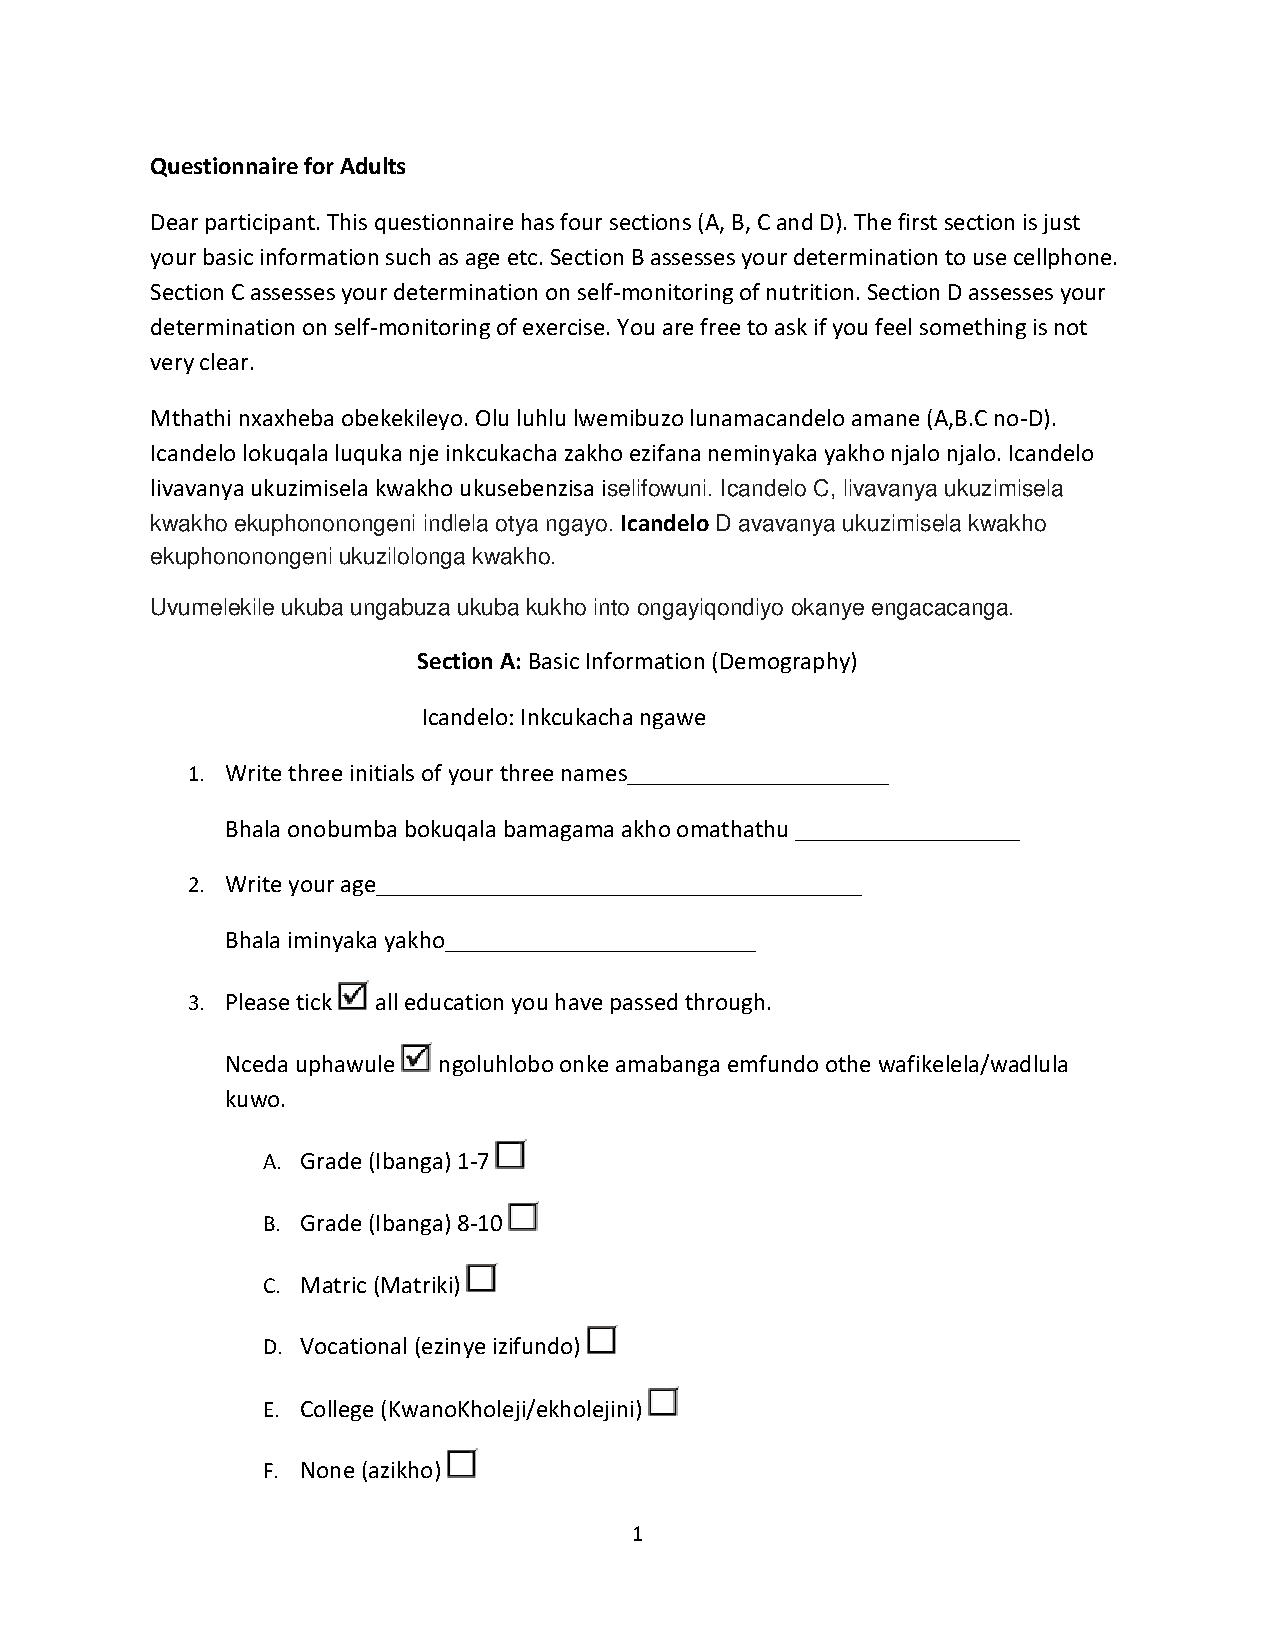
\includepdf[pagecommand={},scale=0.9]{Pdfs/baseline_ben.pdf} 
%\end{center}

%% Appendix A

\chapter{Appendix C. Baseline Questionnaires} % Main appendix title
\clearpage
\label{AppendixC} % For referencing this appendix elsewhere, use \ref{AppendixA}

\lhead{Appendix A. \emph{Baseline Questionnaires}} % This is for the header on each page - perhaps a shortened title
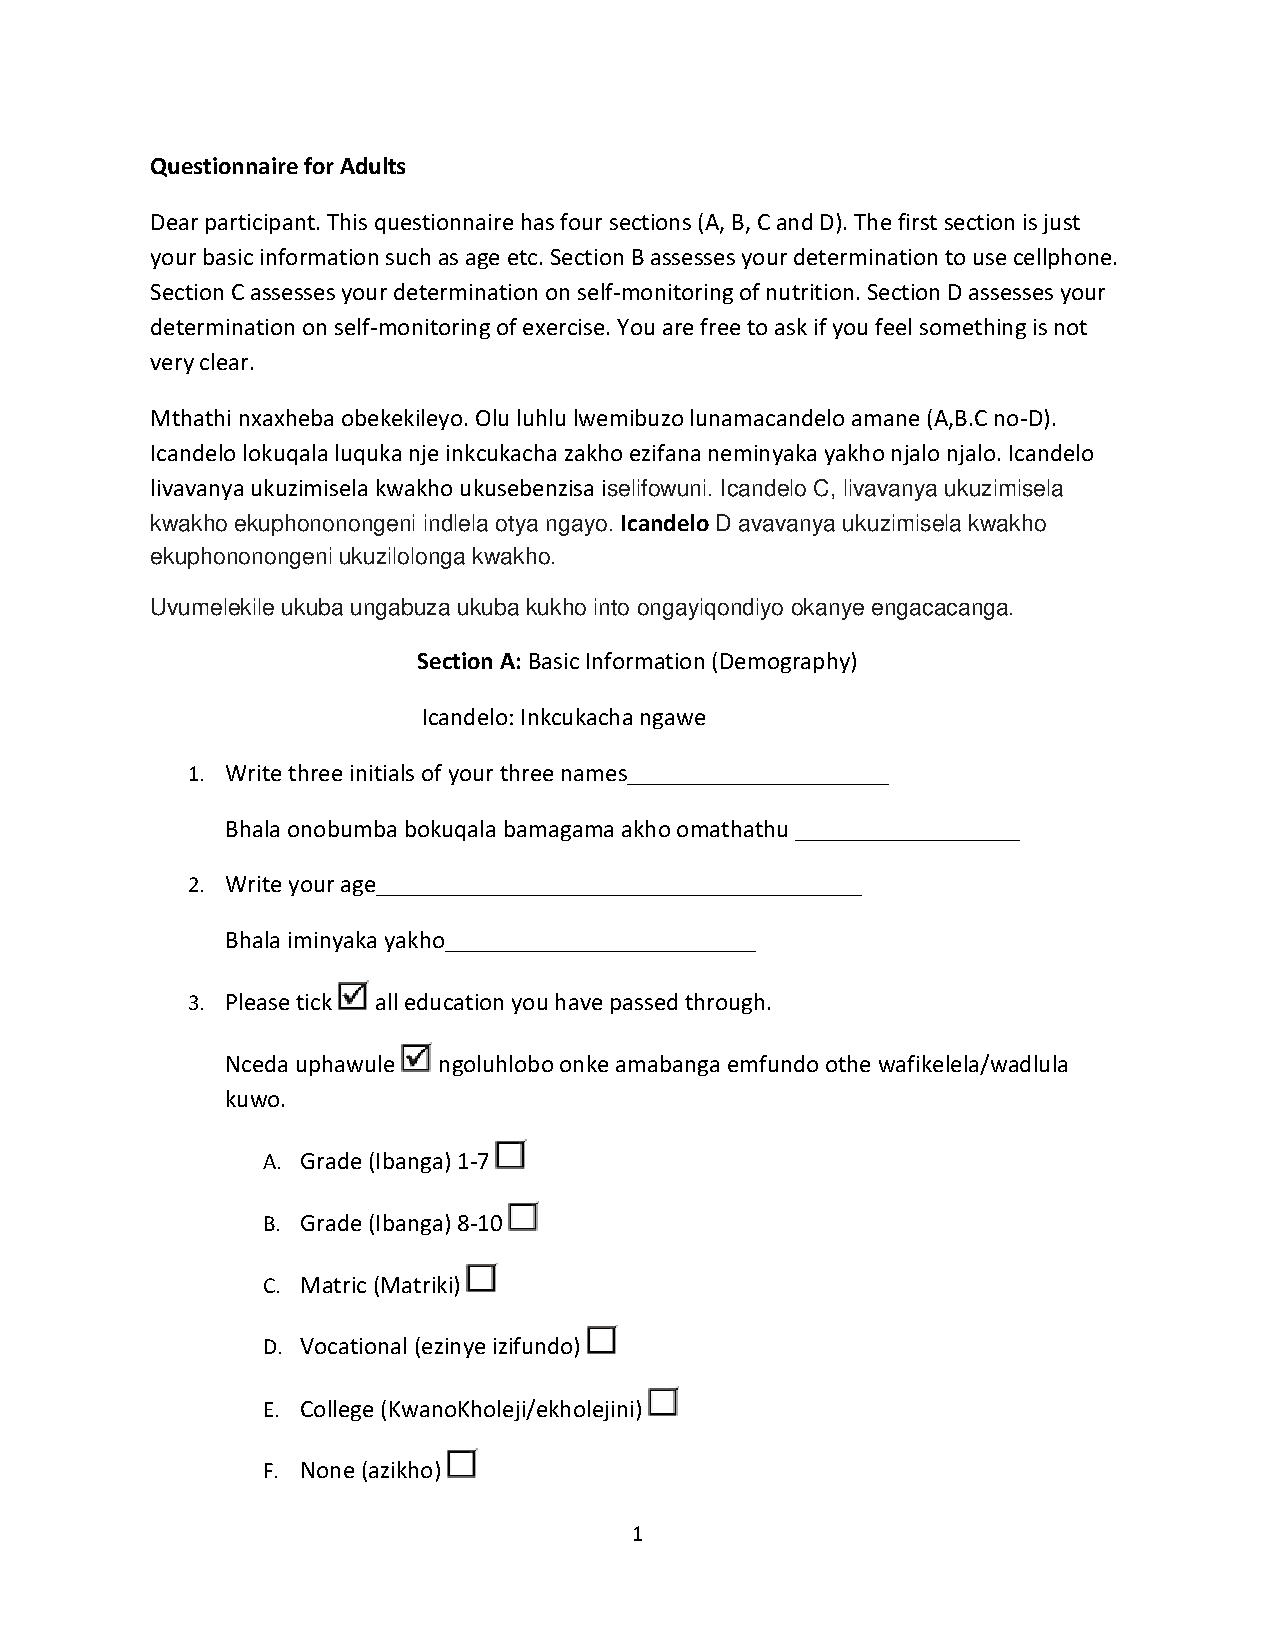
\includepdf[pages=-,frame,pagecommand={},width=\textwidth,offset=90 0]{Pdfs/baseline_ben.pdf}
\clearpage
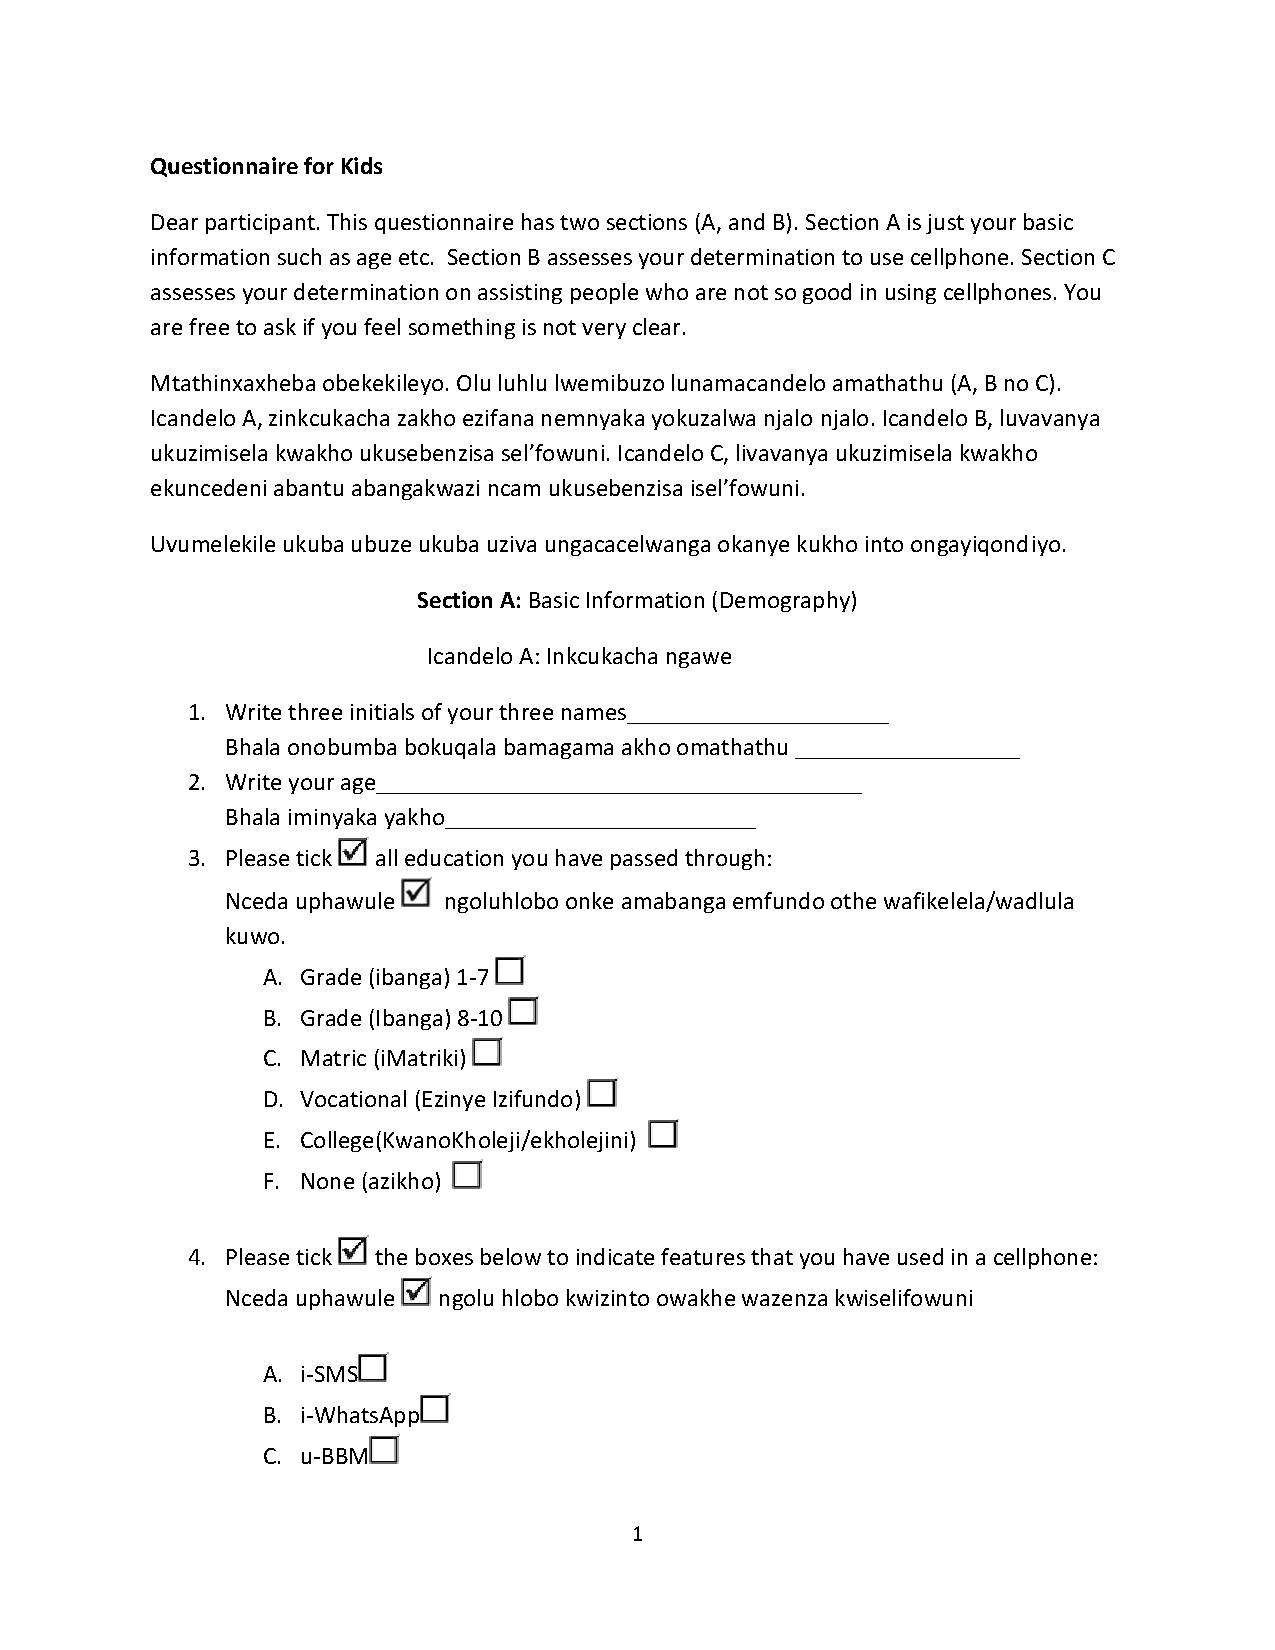
\includepdf[pages=-,frame,pagecommand={},width=\textwidth,offset=90 0]{Pdfs/baseline_interm.pdf}

%\newcommand{\insertrep}[1]{%
%\hspace{-2.4cm}
%\fbox{\includegraphics[page=1,scale=0.8]{#1}}
%\includegraphics[page=1,scale=0.8]{#1}
%\includepdf[scale=0.75,pages=1,frame]{#1}
%}

%\subsection{Interesting Letter}
%\insertrep{Pdfs/baseline_ben.pdf}
%\begin{center}
%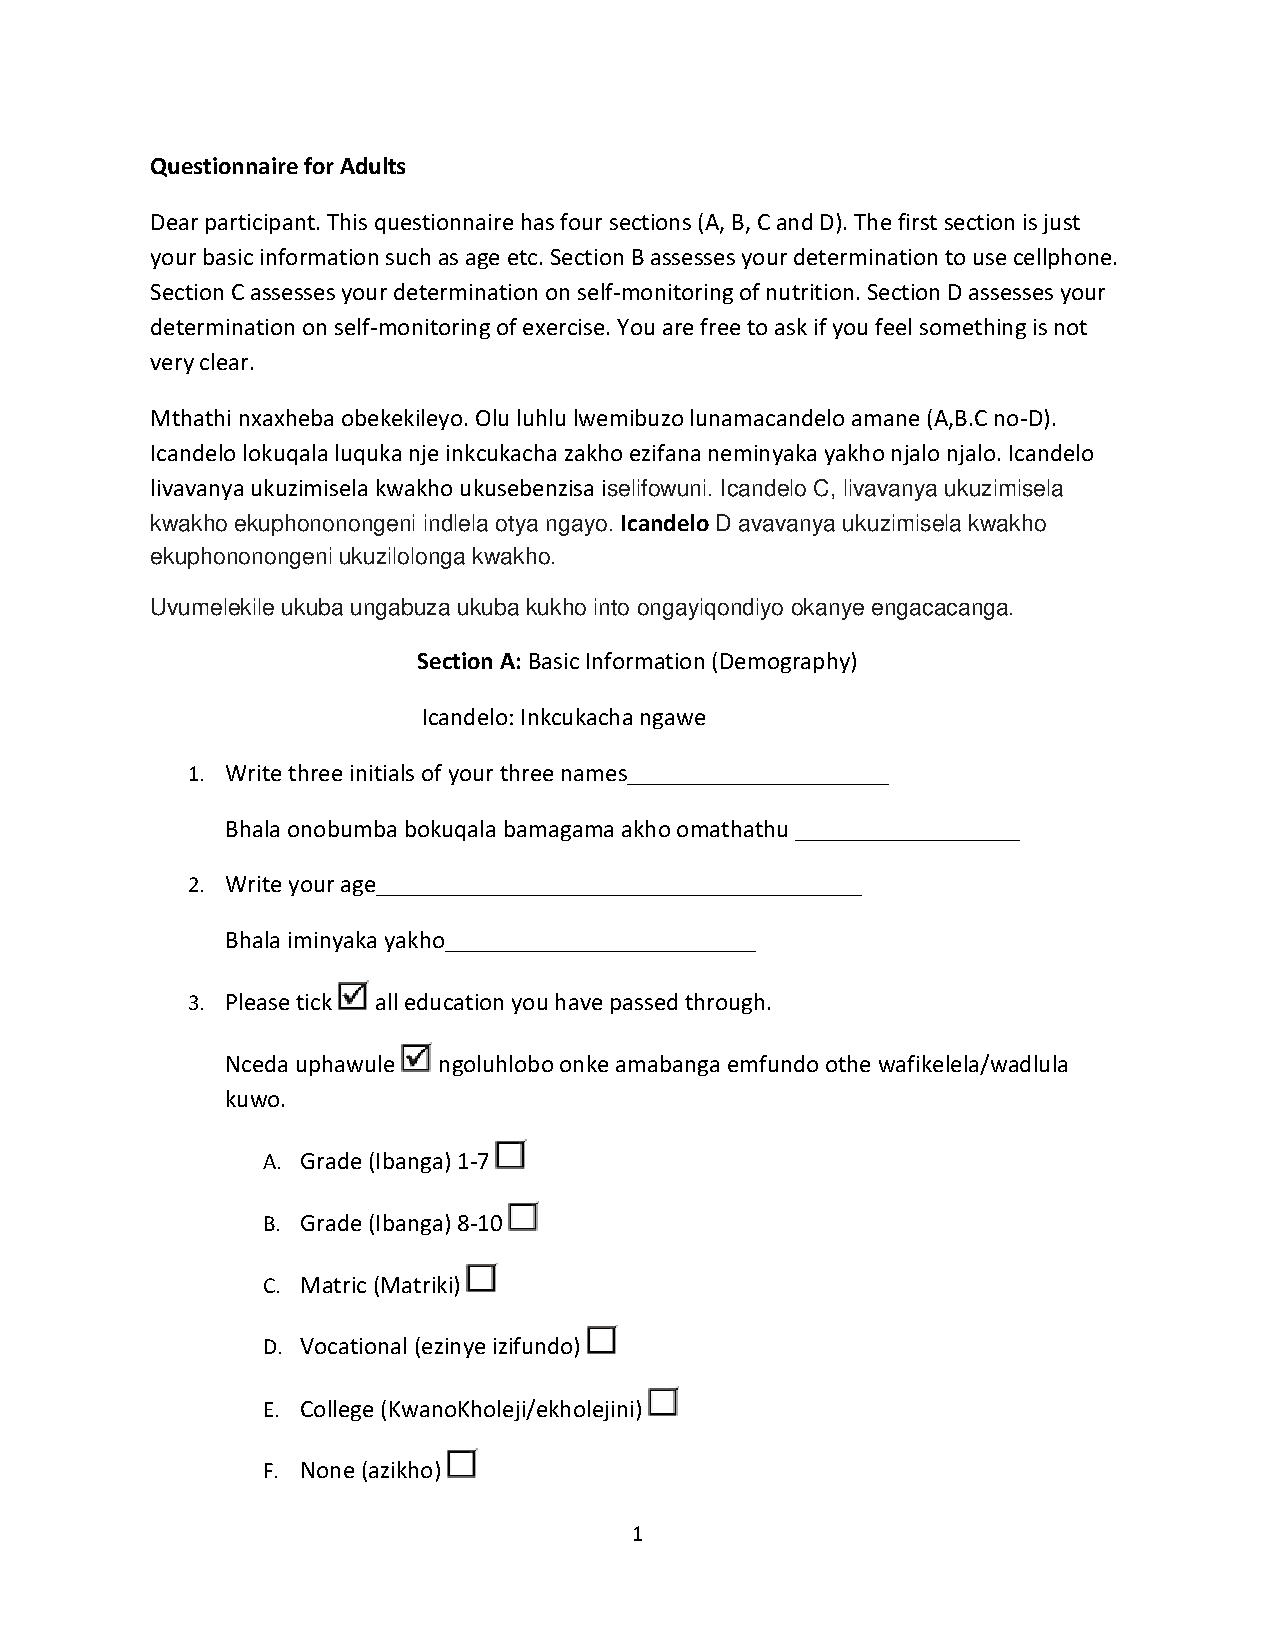
\includepdf[pagecommand={},scale=0.9]{Pdfs/baseline_ben.pdf} 
%\end{center}


\addtocontents{toc}{\vspace{2em}} % Add a gap in the Contents, for aesthetics

\backmatter

%----------------------------------------------------------------------------------------
%	BIBLIOGRAPHY
%----------------------------------------------------------------------------------------

\label{Bibliography}

\lhead{\emph{Bibliography}} % Change the page header to say "Bibliography"

\bibliographystyle{unsrtnat} % Use the "unsrtnat" BibTeX style for formatting the Bibliography

\bibliography{Bibliography} % The references (bibliography) information are stored in the file named "Bibliography.bib"

\end{document}  